\documentclass[10pt]{article}
\usepackage[utf8]{inputenc}
\usepackage{hyperref}
\usepackage{fontenc}
\usepackage{mathptmx}
\usepackage{geometry}
\usepackage{titling}
\usepackage{graphicx}
\usepackage{subcaption}
\setlength{\topskip}{0mm}
\setlength{\droptitle}{-8em} 
\title{{\large \textbf{CONCORDIA UNIVERSITY \\ DEPARTMENT OF COMPUTER SCIENCE AND SOFTWARE ENGINEERING \\ SOEN 6011: SOFTWARE ENGINEERING PROCESSES \\ SECTION CC WINTER 2019 \\ F1: $arccos(x)$}  \\ }}
\author{\normalsize \textbf {STUDENT NAME: YONGCONG LEI} \\ \normalsize \textbf{STUDENT IDENTIFICATION NUMBER: 40045701 }}
\date{}
\begin{document}
\maketitle

\section{Characteristics and Domain}
\subsection{Characteristics}

\begin{enumerate}
    \item $arccos(x)$ is an inverse trigonometric functions of $cos(x)$.
    \item principle values
    \item relationship with $cos(x)$
    \item 
    
    \item $arccos(x)$ is a trigonometric function (relate an angle of a right-angled triangle to ratios of two side lengths).
    \item 
\end{enumerate}

\begin{figure}[h!]
  \centering
  \begin{subfigure}[b]{0.4\linewidth}
    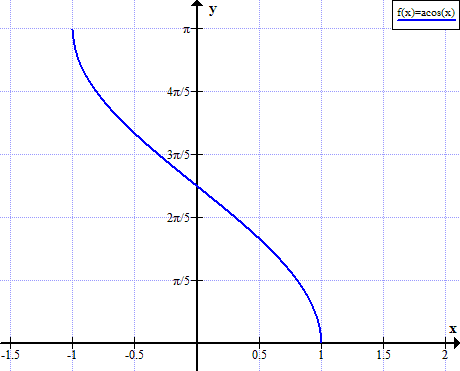
\includegraphics[width=\linewidth]{image/arccos.png}
    \caption{$arccos(x)$}
  \end{subfigure}
  \begin{subfigure}[b]{0.4\linewidth}
    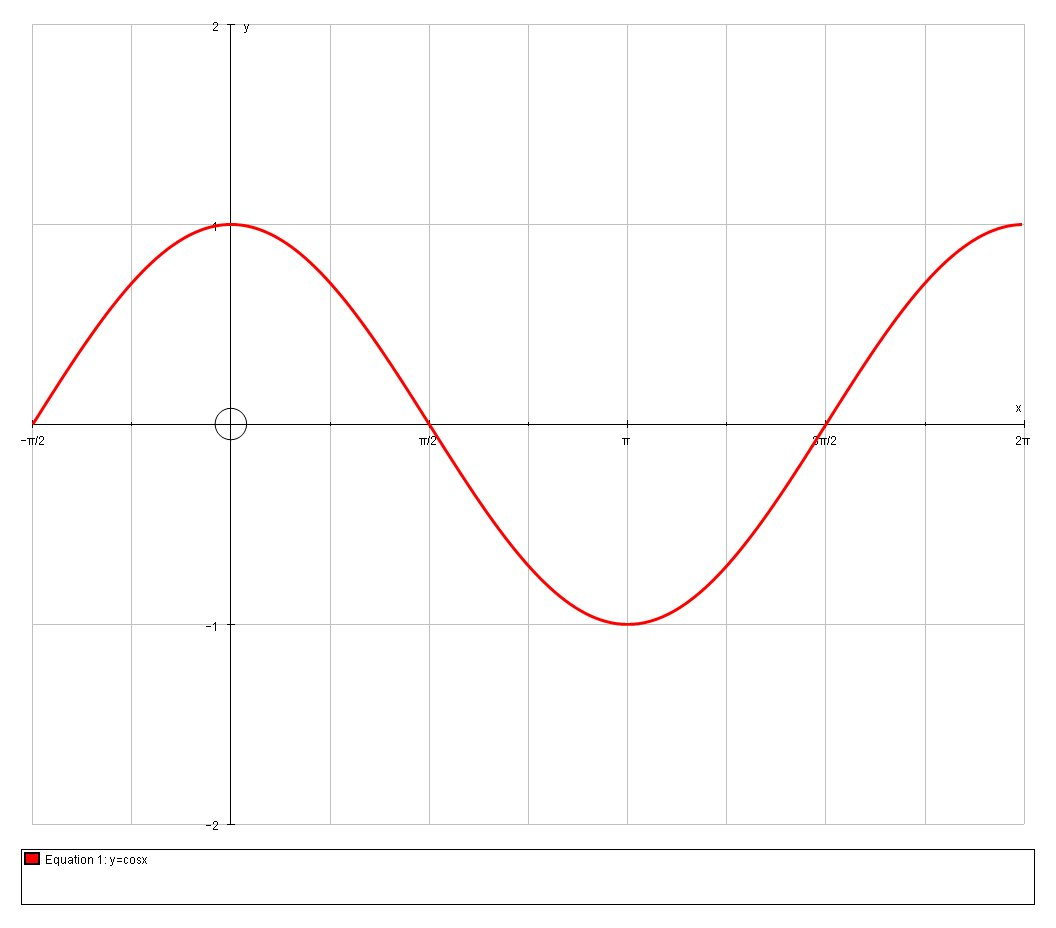
\includegraphics[width=\linewidth]{image/cos.jpg}
    \caption{$cos(x)$}
  \end{subfigure}
  \caption{$arccos(x)$ and $cos(x)$}
  \label{fig:coffee}
\end{figure}

\subsection{Domain and Co-domain}
Assumption: ? \newline
For the equation $y = arccos(x)$, the domain is $x \in [-1, 1]$. 
The co-domain is $y \in [0, \pi]$



\section{Requirements}

\section{Advantages and Disadvantages}

\section{References}
 
\end{document}
